\section{Introduction}

\begin{frame}{Motivation}
\begin{itemize}
    \item Growing importance of efficient last-mile delivery logistics.
    \item Use of drones (Unmanned Aerial Vehicles, UAVs) for overcoming traffic constraints, reducing delivery times, and lowering operational costs.
    \item Significant increase in literature on Delivery Drones in recent years \cite{DUKKANCI2023}.
\end{itemize}
\end{frame}

\begin{frame}{Introduction to Last-Mile Delivery Drones}
    \begin{figure}
      \begin{columns}
        \column{.3\linewidth}
        \caption{Drones Congestion in a high-traffic Last Mile Delivery context. \\ Source: \cite{imageDronesCongestion}}
        \label{fig:example left}
        \column{.65\linewidth}
        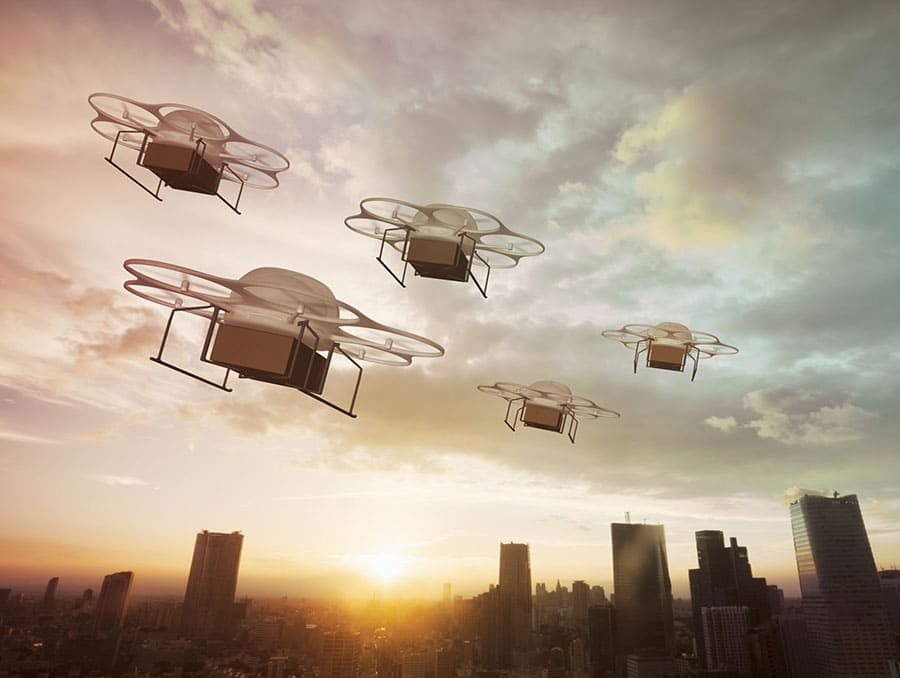
\includegraphics[width=\textwidth]{img/Drone Congestion.jpg}
      \end{columns}
    \end{figure}

\end{frame}

\begin{frame}{Introduction to Last-Mile Delivery Drones}
\destaq{Last Mile Delivery Drones (LMDD)}
\begin{itemize}
    \item Heterogeneous research area:
    \begin{itemize}
        \item Combining drones and trucks.
        \item Linear integer modeling.
        \item Fuzzy logic for uncertainties.
        \item Multi-objective optimization.
        \item Exclusive drone-based solutions.
    \end{itemize}
    \item \textbf{Complex Systems Decentralized Approach}:
    \begin{itemize}
        \item Tradable permit model for multi-agent airspace use \cite{Verri}.
    \end{itemize}
\end{itemize}

\end{frame}

\begin{frame}{Related Work and Centralized Control}
\begin{itemize}
    \item \textbf{Necessity of Air Traffic Management}:
    \begin{itemize}
        \item Most centralized models don't address collision avoidance \cite{DUKKANCI2023}.
        \item Ensuring optimal path planning and efficient airspace control.
    \end{itemize}
    \item \textbf{Centralized Control and UTM}:
    \begin{itemize}
        \item \textbf{Centralized Control}:
        \begin{itemize}
            \item Federal Aviation Administration (FAA) and NASA's Unmanned Aircraft System Traffic Management (UTM) \cite{nasa}.
            \item Ensures organized, legislative-backed airspace control.
        \end{itemize}
        \item \textbf{Decentralized Models}:
        \begin{itemize}
            \item Novel but complex in scalability and regulatory compliance.
        \end{itemize}
    \end{itemize}
\end{itemize}
\end{frame}


\begin{frame}{Proposed Approach}
\begin{itemize}
    \item \textbf{Aispace Control and MAPF Approach}:
    \begin{itemize}
        \item Multi-Agent Path Finding (MAPF) is a solution for addressing spatial characteristics and collision avoidance.
    \end{itemize}
    \item \textbf{Proposed Strategy}:
    \begin{itemize}
        \item Employing MAPF strategy for Last Mile Delivery Drone problem.
        \item Three approaches: MILP, heuristic and hybrid.
        \item Use of prioritized planning \cite{7138650} and conflict-based search \cite{SHARON201540} to manage computational complexity in the heuristic.
        \item Comparing the MILP with the heuristic.
        \item Qualitative comparison between centralized and decentralized approaches.
    \end{itemize}
\end{itemize}
\end{frame}


